 \newpage
 \begin{savequote}[108mm]
``If you expect life to be easy, challenges will seem difficult. If you accept that challenges may occur, life will be easier.''
  \qauthor{Rob Liano}
\end{savequote}
 \chapter{Obstacles that face migration}
 \label{chap:Obstacles}
 \vspace{-2cm}
 Migration is a part of the software life cycle. The concept behind migration is that it should occur as smoothly as possible and without interruption of vital business functions and services.

 Migrating from CSS to FLOSS has its own set of challenge and obstacles. The following will explore some of the challenges and obstacles of migrating to FLOSS. 
 
   \begin{figure}
    \centering
        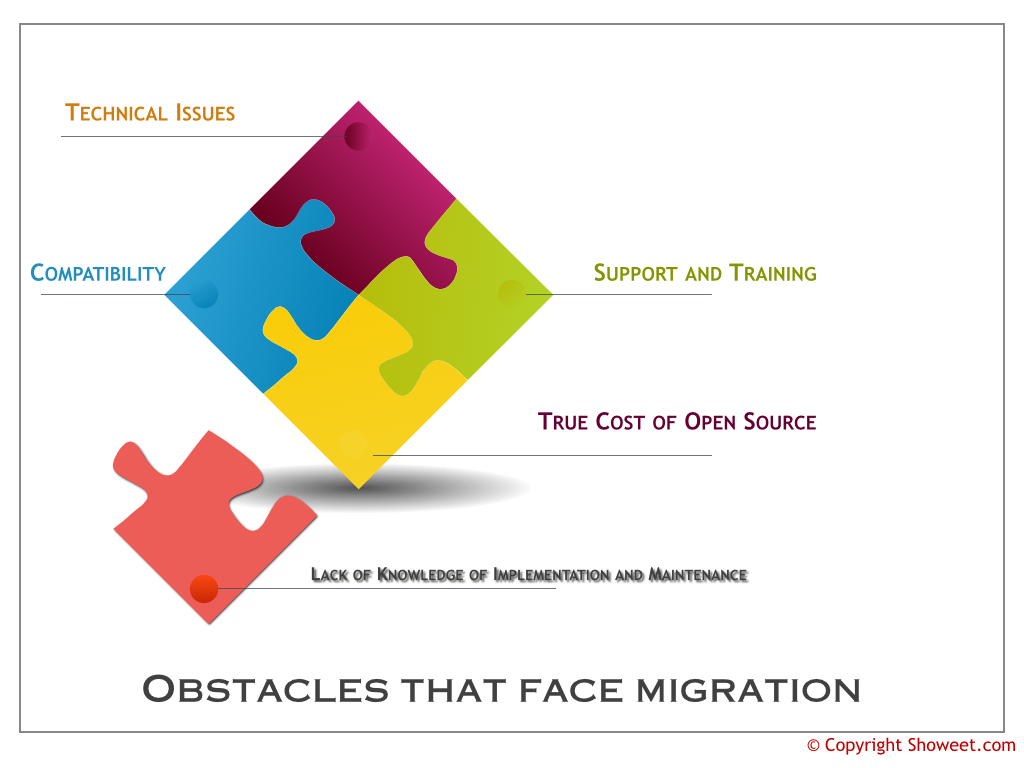
\includegraphics[scale=0.6,angle=90]{img/obsticals.png}
      \caption{Obstacles that face migration}
      \label{fig:Obstacles}
    \end{figure}

 \section{Support and Training}
 \label{sec:Support}


 The migration to FLOSS may be a culture shock to some companies. They will have to get used to resolving problems for themselves, rather than picking up the phone and asking a service representative. However, they also have more freedom to create a software package that is suited to their exact needs. This may be a key advantage for businesses that are in emerging or new areas of business. 

 FLOSS users are often surprised to find the amount of support available from developers and the user community, not to mention how approachable and reasonable the support is. While paid commercial support is ideal for those who need assistance on a regular basis, it is not necessary and is typically only recommended for commercial use. FLOSS ensures that defects are identified and rectified within a timely manner, and as a result of the fact that the software is used by so many, all warranties and liabilities, such as fitness for purpose and merchantability are offered, similar to CSS.  Proprietary vendors typically sell contracts with agreed levels of services, support, or warranties to end users, while FLOSS allows a third party to provide an equal or greater level of support.




 For companies that are used to calling up technical support every time a question or issue arises, the migration to FLOSS may be challenging. Often there is no formal support structure for the system. The advantage is that FLOSS are generally considered easier to administer than CSS. There is usually plenty of information available on open source databases. At worst, the company may have to hire their own expert, which is still cheaper than many CSS licenses. Aside from a lack of support available, there is also no warranty or accountability. This is often and issue with many software migrations. If something goes wrong, the company is on its own. 

 Many companies are choosing to migrate to open source systems such as Linux to free themselves from the increasing financial burdens of Microsoft. A study\footnote{Jashari, Bardhyl and Stojanovski, Filip. Challenges and obstacles: Usage of Free and Open Source Software in local government in Macedonia. Metamorphosis Foundation\label{ftn:Macedonia}} of the migration of government servers Linux  among the governments of local municipalities found that a lack of support was the number one reason why certain municipalities refused to migrate their platforms. This lack of support was a key hindrance to the willingness of municipalities to switch their systems to FLOSS.

 Many companies solved the issue of support by having their own internal team of system administrators and support personnel. Others hired off-site support through hosting and infrastructure partnerships. Some organizations used a combination of these two choices. In larger organizations, there was often a separate division outside of the regular IT department to handle issues with FLOSS migration, programs, and support. The type of system and support set up that worked depended on the size and individual needs of the company.  Even with adding the staff needed to handle maintenance and support functions with the FLOSS, a majority of the companies still reported that the system was a good value for the money.

 \subsection{Training Issues}

 Due to the popularity and familiarity of Windows based systems, many FLOSS platforms have tried to mimic the look and feel of the familiar Windows based systems. However, they are different and the transition can be difficult for some users. Training is needed to overcome many of the user issues associated with the use of the new system. Many municipalities indicated that they would be willing to adopt FLOSS, if training and support were provided. As there is no single entity that accountable for the software, there is no system in place for formal training. Companies that migrate from CSS to FLOSS may need to develop training programs themselves and bear the expense. Having an in-house expert or internal person responsible for support and training may be one solution to overcoming this obstacle.
 
\textit{``There is also another, very human problem to overcome: that most people don't understand computers or software, but have memorized all the keystrokes and mouse-click patterns they need to get through the day, so the second they are given a new program they need to memorize a whole new set.''}\footnote{\url{http://www.largo.com/eGov/apps/document/center.egov?view=item;id=1793}} This can happen any time when new software is introduced in a workplace environment. But train people and answer users' questions will help new users to overcome this difficulties.

 \section{Compatibility}
  Compatibility is an issue in the willingness and success of migration. Government and other large corporate system can have thousands, or even hundreds of thousands of documents and records that they must be able to open on the new system. In the case of moving into Linux, an enterprise has to make sure that whatever software it uses is compatible with the Linux OS.
  The older the version of the CSS, the more prevalent compatibility issues will be. In many cases, the new FLOSS does not only have to be able to open them, they must be able to edit and update them too. These are the key challenges being faced by companies that choose to migrate to FLOSS. 
  A mismatch of programming language and integration is another challenge to the migration to FLOSS. Open source systems can be complex because of the different philosophies and approaches that went into them. Concerns over incompatibility means that the new system may have more bugs than the old one. Being an open source system, these bugs can be corrected by the operators and administrators of the system. However, migrating to a system that has more bugs than the old one is not consistent with the goal of having as few glitches as possible in the migration process. Incompatibility in programming can bring the business to a stop during the migration process. 

  The system is not perfect and not every piece of third party software will run on every system, but it provides many more choices than closed systems.
  Although not all of our favorite programs will run in Linux, the good news is that many of the FLOSS alternatives that have been developed are completely free of charge.


  \section{Technical Issues}
  Aside from compatibility issues linked to the ability to open and edit documents, other technical issues can arise. One of key issues is that proprietary software is often designed to remain proprietary. Reconfiguring the old data can be impossible, because of stop gaps placed in the proprietary software that are intentionally designed to prevent it from being changed. Retooling the old software can be one of the biggest challenges that the company faces. 
  The cost motivation for moving to FLOSS can be compelling, but resolving the technical issues can quickly increase the initial projected costs of the project. Even though technical issues may increase the cost of migration in some cases, it may still be the cheapest route when one take a long term perspective on the cost structure of the project. Using a slower migration approach and breaking the process down into smaller sections can help to mitigate these rising costs. 
	
  \section{Lack of Knowledge of Implementation Procedures and Maintenance}

  A recent study reported that a lack of knowledge of implementation and maintenance issues were one of the reason for failing to migrate to the FLOSS\footnote{Macedonia Survey(Look at Section.\ref{sec:Support}, footnote~\ref{ftn:Macedonia})}. 
  Having a local consultant available to assist with the implementation, maintenance, support, and training issues would make them more willing to complete the migration to FLOSS. These study results may apply to other migrations to FLOSS. This insight may provide solutions in other FLOSS migration circumstances as well.  

  FLOSS takes a team approach to implementation and development. The average user is unfamiliar with the software or possesses the level of expertise necessary to participate in the team environment.
  A lack of oversight in the development of the software is a challenge to the adoption of FLOSS. Uncertainty of the future of the software is another obstacle to the adoption of FLOSS. 

  The lack of a central entity with a unified plan for the future of the development of the software project is a reason for hesitation to migrate.
  There is the possibility that future renditions of the software may not be compatible or useful to the organization.
  Accountability gives managers confidence in the direction of future software upgrades and directions. 
 

 \section{True Cost of FLOSS}
 The ability to have a software package that does not have additional licensing fees and continual costs associated with it may sound enticing, but there are many hidden costs that must be considered before an honest evaluation of the costs of the open source system can be determined. Although FLOSS eliminates many of the additional costs of closed systems, some did not consider them a good value for their money. Some of these reasons were a lack of specific applications, inferior quality, a lack of features, lack of community backing, incomplete implementation, programs that do not work correctly, and complex code bases.
 When the migration is successful, it can save the company money. When interoperability problems, compatibility problems, and system problems plague the new FLOSS, it can end up costing more in the end, negating the savings. If the migration fails completely, then it will cost even more to migrate the system back to the old backbone, representing wasted money and wasted time. Not every migration to FLOSS is successful\footnote{Phipps, S. Triumph and Disaster: Two migrations to Open Office. Open Sources}. Sometimes companies skipped steps and cut costs during the migration in the wrong places. This led to failed migrations and ended up costing the company more in the end. These cases highlight the importance of foreseeing the challenges before the migration and making certain that the migration goes as planned. 
 
 The cost savings and freedom to design as one chooses are key reasons for an upsurge of FLOSS packages. However, a majority of the world is still tied to proprietary software and does not plan to make the switch to FLOSS. 
 

 
 Although this research focuses on the advantages of FLOSS  and promotes it as the preferred solution in many cases, it may not be the solution for everyone, particularly those who are not ready to make the transition. 
 
 FLOSS is often a clone of proprietary software, with enough degrees of difference to satisfy the patent and copyright laws. There is no doubt that there is some functional and well-built open source out on the market today. More is developed on a continual basis. However, FLOSS is still not a replacement for proprietary vendors due to obstacles that it presents. Many versions of FLOSS require a higher level of knowledge than vendor software, making it more challenging than proprietary software. It has been suggested that until more user friendly versions of the software have been developed that FLOSS only be used for back end applications.

 FLOSS faces many challenges that it will need to resolve in order to encourage migration from proprietary systems. 
  The main reasons for this unwillingness to migrate is based on an unwillingness to take on the responsibilities that go along with open source that can be solved by politicians promote and support.
  
  
